\section{Gegenmaßnahmen}
Wie in Abschnitt \ref{explainersub} bereits aufgeführt,
gehören zu einem Buffer-Overflow-Angriff mehrere kombinierte Teile. Wenn
man nun verhindern möchte, dass ein Programm über diesen Angriff gestürzt werden
kann, so hat man mehrere Möglichkeiten diese Teile aufzuhalten oder die Kombination
zu blockieren. Es folgen mehrere Möglichkeiten, grob nach Aufwand (für den Entwickler) sortiert.
\subsection{Übersicht der Maßnahmen}
Low Level:
    \begin{itemize}
        \item Hardware-basierte Lösungen
        \item Betriebssystembasierte Ansätze
    \end{itemize}
Passive Härtung der Programme:
    \begin{itemize}
        \item C Range Error Detector und Out Of Bounds Object
        \item Safe Pointer Instrumentalisierung
        \item Manuelles Buffer-Overflow Blocken (Input-Bereinigung)
    \end{itemize}
Aktive (Analysierende) Lösungen:
    \begin{itemize}
        \item Statische Code-Analyse
        \item Stack-Schutz mit ``Canary'' (Zufallszahl)
    \end{itemize}

\subsection{Canaries}
Die Bezeichnung Canary (Engl. Kanarienvogel) stammt aus der Verwendung der Kanarienvögel als
Indikator für Gas in Mienen. Die Canaries im Code werden als Stack-Schutz verwendet. Das bedeutet,
dass beispielsweise Zufallszahlen im Programm auf dem Stack sind und bei einem Buffer-Overflow-Angriff
überschrieben werden. Ein Tool wie StackGuard kann dann anhand der Änderung einen Fehler feststellen und
die Ausführung des Programms abbrechen.

\subsection{Out Of Bounds Object}
Ein Out Of Bounds Object ist eine Vereinfachte Lösung um Referenzen ungefährlich zu machen.
Es wird verhindert, dass auf Speicher außerhalb des Programms zugegriffen wird, indem Jede
Adresse welche nicht im spezifizierten Bereich liegt auf ein bestimmtes Objekt, das sogenannte
"Out Of Bounds Object" verweist. Dadurch kann innerhalb des laufenden Programms erkannt werden, das
etwas falsch gelaufen ist. Diese Methode ist nicht gängig, da sie technisch gesehen
umgangen werden kann, solange der Angreifer weiß, welcher Speicherbereich für das Programm
vorgesehen ist.


% OS_Based kann schwer zwischen exploit und Intent unterscheiden
% HW_Based gleiches problem

\subsection{Code-Beispiel}
    \begin{center}
        %TODO: Besseres Beispiel finden.
        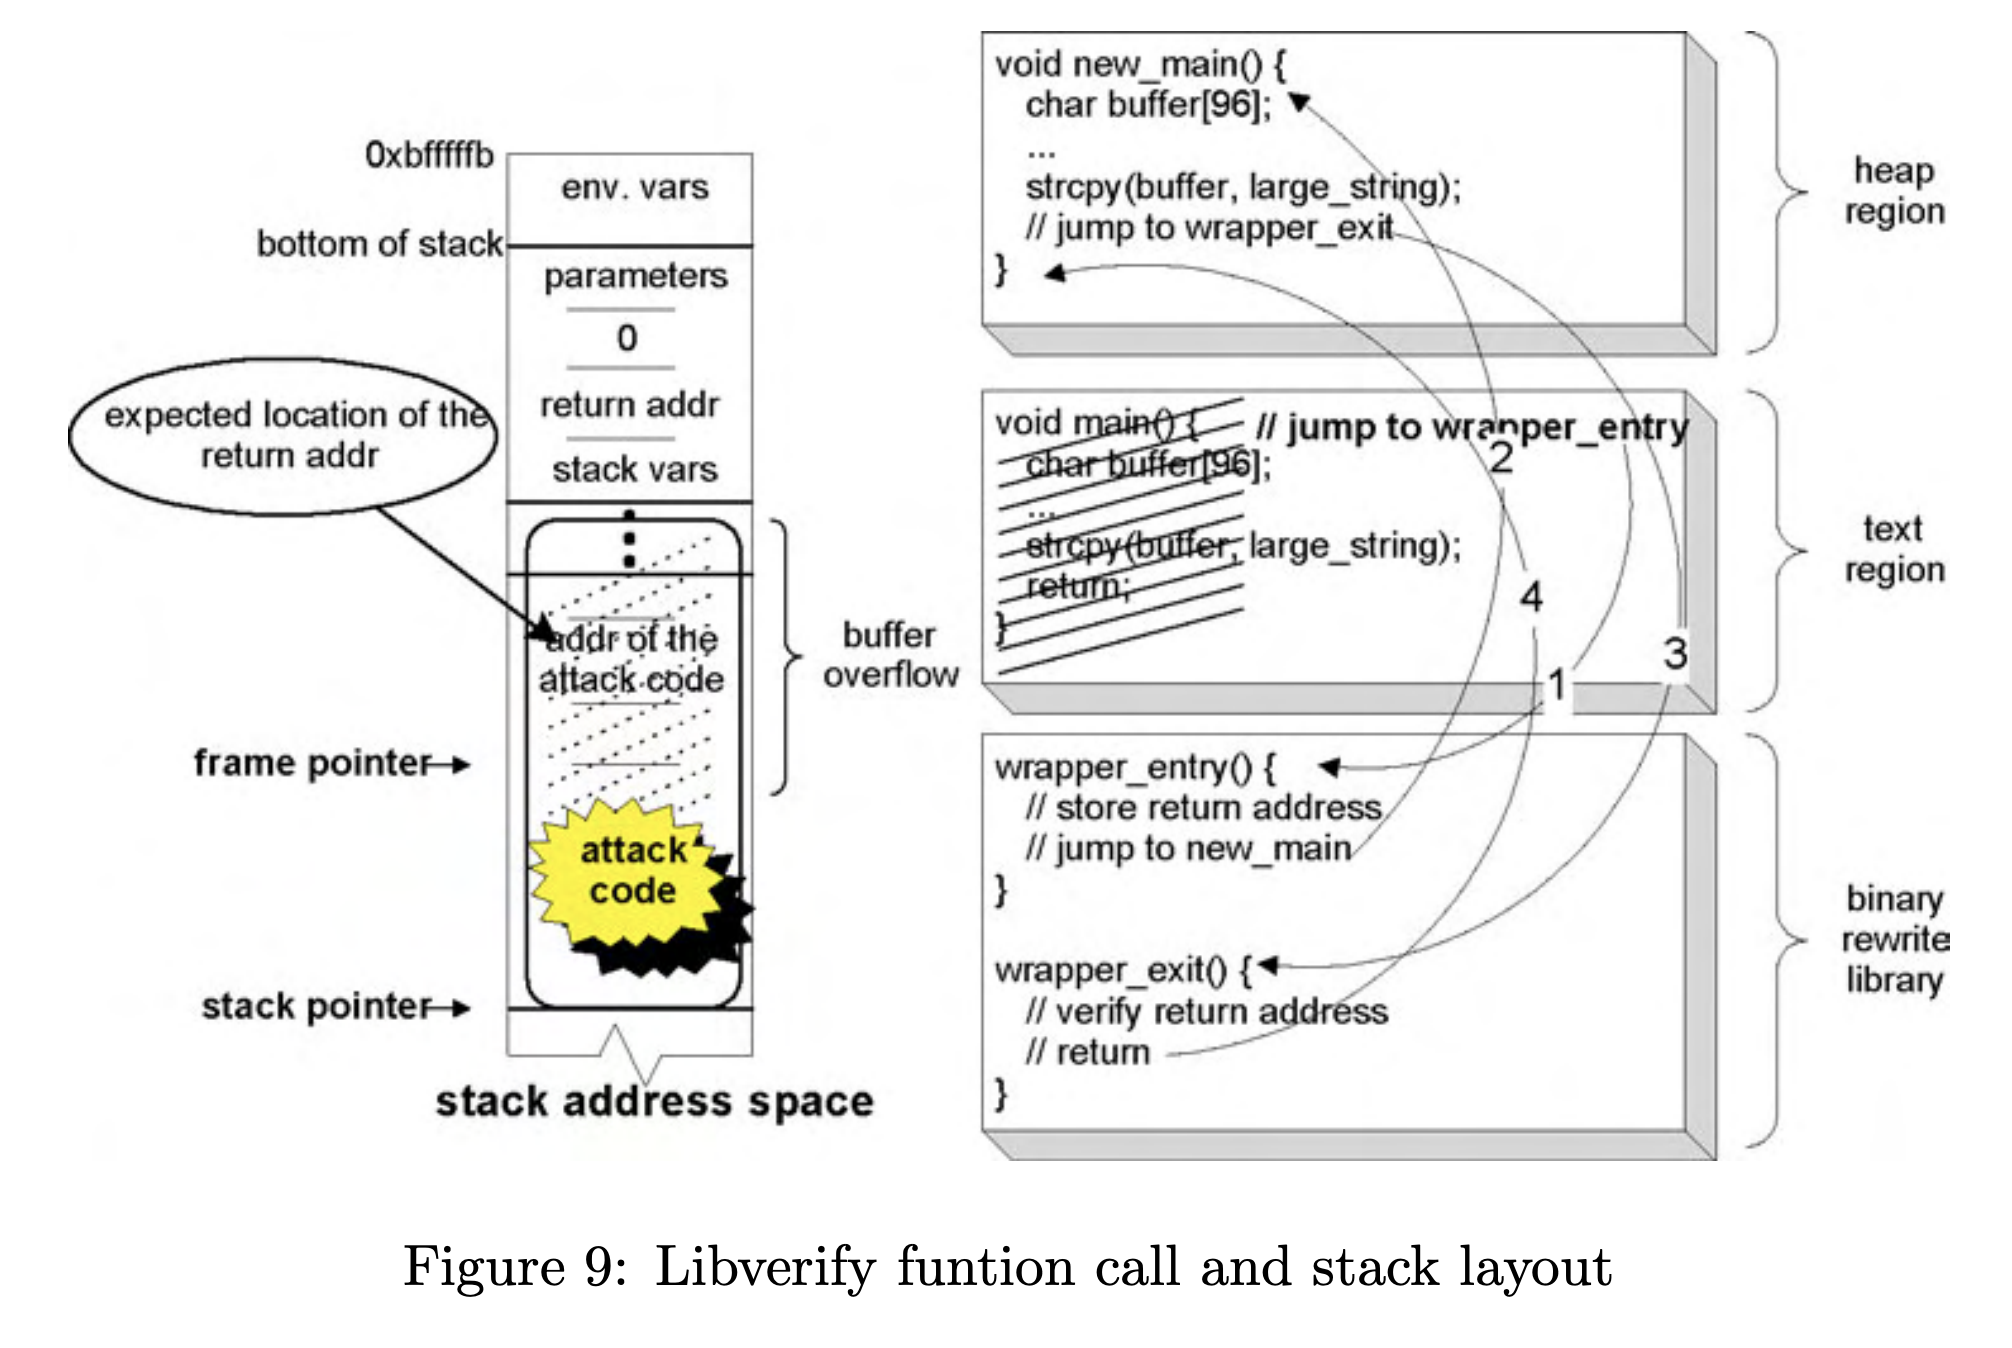
\includegraphics[width=\textwidth,height=0.75\textheight,keepaspectratio]{images/Libverify.png}
    \end{center}

\subsection{Testen}
    \begin{itemize}
        \item Fuzzy Tests
        \item Spezifische Payloads
    \end{itemize}
